\documentclass[a4paper,fleqn,12pt]{article}
\usepackage[utf8]{inputenc}
\usepackage[bulgarian]{babel}
\usepackage{amsmath}
\usepackage{amssymb}
\usepackage{booktabs}
\usepackage{fancyhdr}
\usepackage{amsthm}
\usepackage{graphicx}

%\pagestyle{fancy}
%\fancyhf{}
%\lhead{\rightmark}
%\rhead{\thepage}
%\cfoot{}
%\renewcommand{\headrulewidth}{0pt}


\begin{document}
\begin{titlepage}
	\setlength{\parindent}{0pt}
	\large
\centering
Технически университет -  София \par
Факултет по приложна математика и информатика \par
\vspace{2cm}

{\huge Курсова работа \par}

\vspace{2cm}

\vspace{1cm}
{\LARGE\scshape  Математическа Екология \par}



\vfill

\begin{minipage}[t]{.5\linewidth}
	Студент: \\
	Кристиян Кръчмаров
\end{minipage}%
\begin{minipage}[t]{.5\linewidth}
	\raggedleft
	Преподавател:\\
	проф. дмн. Людмил Каранджулов
\end{minipage}

\vspace{2cm}
\raggedright

\end{titlepage}
\tableofcontents
\newpage
%\fontsize{14pt}{16pt}\selectfont
\section{Задание}
За математическия модел на съжителство на две популации
\begin{gather*}
		\begin{array}{|l@{}} \tag{$\ast$}
		\dot{N_1} = \left(a - bN_1 - \sigma N_2 \right) N_1 \qquad a,b,\sigma > 0\\
		\dot{N_2} = \left(c - \nu N_1 - d N_2 \right) N_2 \qquad c,d,\nu > 0 \\
		\end{array} \\
\text{са въведени следните означения} \\
\Delta = \begin{vmatrix}b & \sigma \\ \nu & d \end{vmatrix} \qquad 
\Delta_1 = \begin{vmatrix}a & \sigma \\ c & d \end{vmatrix} \qquad 
\Delta_2 = \begin{vmatrix}b & a\\ \nu & c \end{vmatrix}
\end{gather*}
Изследвайте вида на особенните точки, 
фазова картина, компютърна реализация, 
съответни чертежи и биологични изводи, ако е изпълнено
	\begin{equation*}
	\Delta > 0 \qquad \Delta_1 > 0 \qquad \Delta_2 > 0
	\end{equation*}

\newpage
\section{Решение}
\subsection{Особенни точки}
Oсобенните точки се получават като решение на системата
\begin{gather*}
		\begin{array}{|l@{}}
		\left(a - bN_1 - \sigma N_2 \right) N_1 = 0\\
		\left(c - \nu N_1 - d N_2 \right) N_2 = 0 \\
		\end{array}
\end{gather*}

\subsubsection{Първи случай}
\begin{gather*}
	\begin{array}{|l@{}}\tag{$I$}
		 N_1 = 0\\
		 N_2 = 0
	\end{array}
\end{gather*}
\subsubsection{Втори случай}
\begin{gather*}
	\begin{array}{|l@{}}\tag{$II$}
		 N_1 = 0\\
		 N_2 \neq 0
	\end{array} \implies c - dN_2 = 0 \implies 
	\begin{array}{|l@{}}
		 N_1 = 0\\
		 N_2 = \frac{c}{d}
	\end{array}
\end{gather*}
\subsubsection{Трети случай}
\begin{gather*}
	\begin{array}{|l@{}}\tag{$III$}
		 N_1 \neq 0\\
		 N_2 = 0
	\end{array} \implies a- bN_1 = 0 \implies 
	\begin{array}{|l@{}}
		 N_1 = \frac{a}{b}\\
		 N_2 = 0
	\end{array} 
\end{gather*}
\subsubsection{Четвърти случай}
\begin{gather*}
	\begin{array}{|l@{}}
		 N_1 \neq 0\\
		 N_2 \neq 0 
	\end{array} \implies 
	\begin{array}{|l@{}}
		a - bN_1 - \sigma N_2 = 0\\
		c - \nu N_1 - d N_2  = 0
	\end{array} \iff 
		\begin{array}{|l@{}}
		 bN_1 + \sigma N_2 = a\\
		\nu N_1 + d N_2  = c
	\end{array}\implies \\
	\begin{array}{|l@{}}\tag{$IV$}
		 N_1 = \frac{\Delta_1}{\Delta} \\
		 N_2 = \frac{\Delta_2}{\Delta}
	\end{array} \qquad \text{(Крамер)} 
\end{gather*}

\subsection{Линеаризация}
Линеаризацията се получава като се замести в ($\ast$)
\begin{gather*}
	\begin{array}{|l@{}}
		 N_1 - \alpha = y_1\\
		 N_2 - \beta = y_2 
	\end{array} \iff
	\begin{array}{|l@{}}
		 N_1 =  y_1 + \alpha\\
		 N_2= y_2 + \beta
	\end{array}
\end{gather*}
където $(\alpha, \beta)$ е особенна точка и се вземе линейната част за всяка една променлива $y_1, y_2$
\subsubsection{Първи случай}
\begin{gather*}
	\begin{array}{|l@{}}
		 N_1 - 0 = y_1\\
		 N_2 - 0 = y_2
	\end{array} \iff 
	\begin{array}{|l@{}}
		 N_1 = y_1\\
		 N_2 = y_2
	\end{array} \implies
	\begin{array}{|l@{}}
		\dot{y_1} = \left(a - by_1 - \sigma y_2 \right) y_1\\
		\dot{y_2} = \left(c - \nu y_1 - d y_2 \right) y_2 
	\end{array} \iff \\ \\
	\begin{array}{|l@{}}
		\dot{y_1} = ay_1 - by_1 ^2- \sigma y_1 y_2 \\
		\dot{y_2} = cy_2 - \nu y_1y_2 - d y_2 ^2 
	\end{array} 
\implies  W = \begin{pmatrix} a&0\\0&c \end{pmatrix} \tag{$I$}
\end{gather*}
\subsubsection{Втори случай}
\begin{gather*}
	\begin{array}{|l@{}}
		 N_1 - 0 = y_1\\
		 N_2 - \frac{c}{d}= y_2
	\end{array} \iff 
	\begin{array}{|l@{}}
		 N_1 = y_1\\
		 N_2 = y_2 + \frac{c}{d}
	\end{array} \implies
	\begin{array}{|l@{}}
		\dot{y_1} = \left[a - by_1 - \sigma \left(y_2 + \frac{c}{d} \right) \right] y_1\\
		\dot{y_2} = \left[c - \nu y_1 - d \left(y_2 + \frac{c}{d} \right) \right] \left(y_2 + \frac{c}{d} \right) 
	\end{array} \iff \\ \\
	\begin{array}{|l@{}}
		\dot{y_1} = ay_1 - by_1 ^2- \sigma y_1 y_2 - \frac{\sigma c}{d} y_1\\
		\dot{y_2} = \left[c - \nu y_1 - dy_2 -c \right] \left(y_2 + \frac{c}{d} \right)  
	\end{array} \iff 
	\begin{array}{|l@{}}
		\dot{y_1} = ay_1 - by_1 ^2- \sigma y_1 y_2 - \frac{\sigma c}{d} y_1\\
		\dot{y_2} =\nu y_1 y_2 - \frac{\nu c}{d} y_1 - dy_2 ^2 - cy_2
	\end{array}
	\implies \\ \\ 
	W = \begin{pmatrix} a - \frac{\sigma c}{d}&0\\- \frac{\nu c}{d}& -c  \end{pmatrix} \tag{$II$}
\end{gather*}

\subsubsection{Трети случай}
\begin{gather*}
	\begin{array}{|l@{}}
		 N_1 - \frac{a}{b} = y_1\\
		 N_2 - 0 = y_2
	\end{array} \iff 
	\begin{array}{|l@{}}
		 N_1 = y_1 + \frac{a}{b} \\
		 N_2 = y_2
	\end{array} \implies
	\begin{array}{|l@{}}
		\dot{y_1} = \left[a - b \left(y_1 + \frac{a}{b} \right) - \sigma y_2 \right] \left(y_1 + \frac{a}{b} \right)\\
		\dot{y_2} = \left[c - \nu \left(y_1 + \frac{a}{b} \right) - dy_2 \right] y_2 
	\end{array} \iff \\ \\
	\begin{array}{|l@{}}
		\dot{y_1} = \left[a - b y_1 -a - \sigma y_2 \right] \left(y_1 + \frac{a}{b} \right)\\
		\dot{y_2} =  c y_2 - \nu y_1 y_2 - \frac{\nu a}{b}- dy_2  ^2  
	\end{array} \iff 
	\begin{array}{|l@{}}
		\dot{y_1} = - b y_1 ^2 - ay_1 - \sigma y_1 y_2 - \frac{\sigma a}{b} \\
		\dot{y_2} =  c y_2 - \nu y_1 y_2 - \frac{\nu a}{b}- dy_2  ^2  
	\end{array}
	\implies \\ \\ 
	W = \begin{pmatrix} -a & - \frac{\sigma a}{b}\\0& c - \frac{\nu a}{b} \end{pmatrix} \tag{$III$}
\end{gather*}
\subsubsection{Четвърти случай}
\begin{gather*}
	\begin{array}{|l@{}}
		 N_1 - \frac{\Delta_1}{\Delta} = y_1 \\
		 N_2 - \frac{\Delta_2}{\Delta} = y_2
	\end{array} \iff 
	\begin{array}{|l@{}}
		 N_1  = y_1 + \frac{\Delta_1}{\Delta}\\
		 N_2  = y_2 + \frac{\Delta_2}{\Delta}
	\end{array} \implies
	\begin{array}{|l@{}}
		\dot{y_1} = \left[a - b \left(y_1 + \frac{\Delta_1}{\Delta} \right) - \sigma \left(y_2 + \frac{\Delta_2}{\Delta} \right)\right] \left(y_1 + \frac{\Delta_1}{\Delta} \right)\\
		\dot{y_2} = \left[c - \nu \left(y_1 + \frac{\Delta_1}{\Delta} \right) - d \left(y_2 + \frac{\Delta_2}{\Delta} \right) \right] \left(y_2 + \frac{\Delta_2}{\Delta} \right)
	\end{array} \\ \\
\begin{array}{|l@{}}
		\dot{y_1} = \left[a-by_1-\frac{b\Delta_1}{\Delta} - \sigma y_2 - \frac{\sigma\Delta_2}{\Delta} \right] 
					\left(y_1 + \frac{\Delta_1}{\Delta} \right) \\
		\dot{y_2} = \left[c - \nu y_1 - \frac{\nu\Delta_1}{\Delta} -dy_2 - \frac{d\Delta_2}{\Delta}\right] 
					\left(y_2 + \frac{\Delta_2}{\Delta} \right)
	\end{array} \iff \\ \\
	\begin{array}{|l@{}}
		\dot{y_1} =  ay_1 + \frac{a\Delta_1}{\Delta} -by_1 ^2 - \frac{b\Delta_1}{\Delta}y_1 - \frac{b\Delta_1}{\Delta}y_1 
					- b \left( \frac{\Delta_1}{\Delta}\right)^2  - \sigma y_1 y_2 - \frac{\sigma\Delta_1}{\Delta} y_1
					- \frac{\sigma\Delta_2}{\Delta} y_1 - \frac{\sigma\Delta_1\Delta_2}{\Delta^2}\\
		\dot{y_2} = cy_2 + \frac{c\Delta_2}{\Delta} - \nu y_1y_2 -  \frac{\nu\Delta_2}{\Delta}y_1 
					-  \frac{\nu\Delta_1}{\Delta}y_2 - \frac{\nu\Delta_1\Delta_2}{\Delta^2}
					- d y_2 ^2 -  \frac{d\Delta_2}{\Delta}y_2 - \frac{d\Delta_2}{\Delta}y_2 
					- d\left( \frac{\Delta_2}{\Delta}\right)^2 
	\end{array} \implies \\ \\ 
	W = \begin{pmatrix}
 			a -\frac{2b\Delta_1}{\Delta} - \frac{\sigma\Delta_2}{\Delta}& - \frac{\sigma \Delta_1}{\Delta}\\
			- \frac{\nu\Delta_2}{\Delta}& c - \frac{2d \Delta_2}{\Delta} - \frac{\nu\Delta_1}{\Delta}
		 \end{pmatrix}
\end{gather*}
\begin{gather*}
W = \frac{1}{\Delta}  
		\begin{pmatrix}
 			\Delta a - 2b\Delta_1 - \sigma\Delta_2 & - \sigma \Delta_1\\
			- \nu\Delta_2& \Delta c - 2d \Delta_2 - \nu\Delta_1
		 \end{pmatrix} \\
\Delta a - 2b\Delta_1 - \sigma\Delta_2 = (bd - \nu\sigma)a - 2b(ad-c\sigma) - \sigma(bc-a\nu) = \\
abd-a\nu\sigma - 2abd +2bc\sigma - bc\sigma + a\nu\sigma = bc\sigma - abd = b(c\sigma - ad) = -b(ad-c\sigma) = -b\Delta_1 \\ \\
\Delta c - 2d \Delta_2 - \nu\Delta_1 = (bd-\nu\sigma)c - 2d(bc-a\nu) - \nu(ad-c\sigma) = \\
bcd - c\nu\sigma - 2bcd + 2ad\nu - ad\nu + c\nu\sigma = ad\nu-bcd = d(a\nu-bc) = -d(bc- a\nu) = -d\Delta_2 \\
\implies W = -\frac{1}{\Delta} \begin{pmatrix} b\Delta_1 & \sigma\Delta_1 \\ \nu\Delta_2 & d\Delta_2 \end{pmatrix} \tag{$IV$} 
\end{gather*}

%\begin{gather*}
%	W = \frac{1}{\Delta} \begin{pmatrix} b\Delta_1 & \sigma\Delta_1 \\ \nu\Delta_2 & d\Delta_2 \end{pmatrix} \text{?!?!}
%\end{gather*}

\subsection{Собствени стойностти}
Собствените стойностти на матрицата $W$ се получават от уравнението
$$\det(W-\lambda I) = 0$$
където $I$ е единичната матрица
\subsubsection{Първи случай}
\begin{gather*}
	\det(W-\lambda I)  = \begin{vmatrix} a-\lambda&0\\0&c - \lambda \end{vmatrix} = (a-\lambda)(c - \lambda)=0 \implies 	\\
	\begin{array}{|l@{}}
		 \lambda_1 =  a > 0\\
		 \lambda_2 = c > 0
	\end{array} \tag{$I$} \implies  \text{ неустойчив възел}
\end{gather*}
\subsubsection{Втори случай}
\begin{gather*}
	\det(W-\lambda I)  = 
	\begin{vmatrix}
		 a - \frac{\sigma c}{d} - \lambda &0\\
		- \frac{\nu c}{d}& -c   -\lambda
	\end{vmatrix} = 
		\left(\frac{ad - \sigma c}{d} - \lambda \right)(- c - \lambda)=0 \implies \\ \\
	\begin{array}{|l@{}}
		 \lambda_1 =  \frac{ad - \sigma c}{d} = \frac{\Delta_1}{d} > 0\\
		 \lambda_2 = -c < 0
	\end{array} \tag{$II$} \implies  \text{седло}
\end{gather*}
\subsubsection{Трети случай}
\begin{gather*}
 \det(W-\lambda I)  = 
	\begin{vmatrix}
		-a-\lambda & - \frac{\sigma a}{b}\\
		0& c - \frac{\nu a}{b} - \lambda
	\end{vmatrix} = 
		(-a - \lambda) \left( \frac{bc - \nu a}{b} - \lambda \right)=0 \implies \\ \\
	\begin{array}{|l@{}}
		 \lambda_1 =  \frac{bc - \nu a}{b} = \frac{\Delta_2}{d} > 0\\
		 \lambda_2 = -a < 0
	\end{array} \tag{$III$} \implies  \text{ седло}
\end{gather*}
\subsubsection{Четвърти случай}
\begin{gather*}
 \det(W-\lambda I)  = 
	\begin{vmatrix}
		 b\Delta_1 -\lambda & \sigma\Delta_1 \\
		 \nu\Delta_2 & d\Delta_2 - \lambda
	\end{vmatrix} = 
		(b\Delta_1 - \lambda) (d\Delta_2 - \lambda) -  \nu\sigma\Delta_1\Delta_2 =0 \iff \\ \\
		bd\Delta_1\Delta_2-b\Delta_1\lambda - d\Delta_2\lambda+\lambda^2 -  \nu\sigma\Delta_1\Delta_2 =0 \iff \\ \\
		\lambda^2 - \lambda (b\Delta_1 + d\Delta_2) + \Delta_1\Delta_2 (bd-\nu\sigma) = 0 \iff 
		\lambda^2 - \lambda (b\Delta_1 + d\Delta_2) + \Delta \Delta_1\Delta_2 = 0 \\
		\\
		\text{Формули на Виет : } p\lambda^2 + q\lambda + r\\
		\begin{array}{|l@{}}
		\lambda_1 + \lambda_2 = - \frac{q}{p} = - (b\Delta_1 + d\Delta_2) < 0\\
		\lambda_1 \cdot \lambda_2 = \frac{r}{p} = \Delta \Delta_1\Delta_2 > 0
		\end{array} \\
\implies   \lambda_{1,2} = \alpha \pm \beta i \in \mathbb{C}, \alpha < 0 \implies \text{ фокус} \tag{$IV$} 
\end{gather*}

\newpage
\subsection{Фазова картина}




\newpage
\subsection{Компютърна реализация}
Следния код реализира модела на съжителство в Matlab
\begin{verbatim}
function ecologyGraph(a,b,sigma,c,nu,d,N0,i)
% Дефиниране интервала на времето
tspan = [0 100];

% Дефиниране на функцията, която описва системата
ode = @(t, N) [ (a - b*N(1) - sigma*N(2)) * N(1);
                (c - nu*N(1) - d*N(2)) * N(2)];

% Решаване на системата от диференциални уравнения
[t, N] = ode45(ode, tspan, N0);

% Визуализация на резултатите
figure(i),plot(t, N(:,1), 'r-', t, N(:,2), 'b--');
legend('N_1', 'N_2', 'Location' , 'best');
xlabel('Time');
ylabel('Population');
end
\end{verbatim}
Този код представлява функция, която генерира графика на две популационни групи в зависимост от времето. 
Функцията има следните параметри:
\begin{itemize}    
	\item $a,b,\sigma, c, \nu, d$ - коефициенти определящи растежа на популацията. 
	\item $N_0$ - началните стойности на популациите във формата $[N_1(0), N_2(0)]$
	\item $i$ - номер на графиката, която ще бъде създадена
\end{itemize}
Функцията използва система от диференциални уравнения, описваща динамиката на популационните групи. 
Тези уравнения се задават в функцията ode, която приема два аргумента: време t и вектор N, който съдържа стойностите на популациите на двата вида.\\
След това се използва вградената MATLAB функция ode45, която решава системата от диференциални уравнения, зададени в ode, в интервала на времето tspan, като използва началните стойности $N_0$. \\
След като решението на системата от диференциални уравнения е генерирано, функцията визуализира резултатите чрез графика на две криви, които показват стойностите на популациите на двата вида във времето.  

\newpage
\subsection{Примери}
\subsubsection*{Пример 1}
\begin{gather*}
	\begin{array}{|l@{}}
	\dot{N_1} = \left(5 - 2N_1 - 2 N_2 \right) N_1 \qquad N_1(0) = 1\\
	\dot{N_2} = \left(3 - 1N_1 - 6 N_2 \right) N_2  \qquad N_2(0) = 1
	\end{array} \\
	\Delta = \begin{vmatrix} 2 & 2 \\ 1 & 6 \end{vmatrix} = 12 - 2 = 10 > 0 \\
	\Delta_1 = \begin{vmatrix}5 & 2 \\ 3 & 6 \end{vmatrix} = 30 - 6 = 24 > 0 \\
	\Delta_2 = \begin{vmatrix}2 & 5\\ 1 & 3 \end{vmatrix} = 6-5 = 1 > 0
\end{gather*}
Кодът от предходната част генерира следната графика: \\
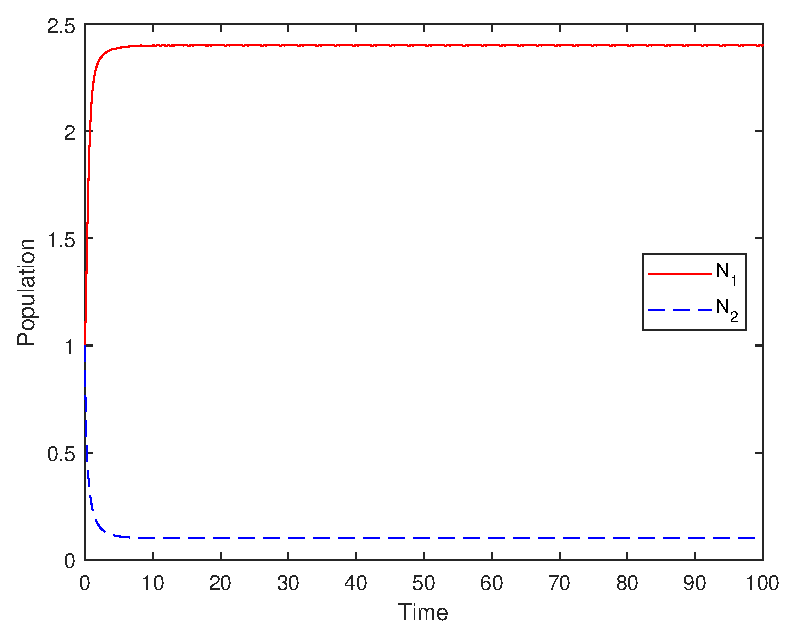
\includegraphics [width=4in]{ecologyComp_01.eps} \\
Както се вижда от графиката и двете популации запазват своя брой константен във времето. \\
Забелязва се, че $N_1$ е със стойност $2.4 = \frac{\Delta_1}{\Delta}$. \\
Аналогично за $N_2$ стойността е $0.1 = \frac{\Delta_2}{\Delta}$. \\
\newpage
\begin{figure}[htp!]
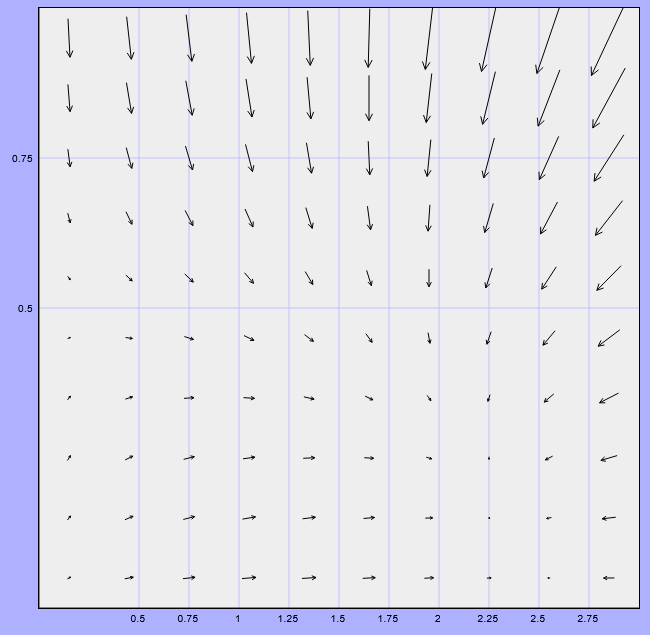
\includegraphics [width=6in]{fazof-portret-primer-1.png}
\caption{Фазов портет}
\end{figure}

\newpage
\subsubsection*{Пример 2}
\begin{gather*}
	\begin{array}{|l@{}}
	\dot{N_1} = \left(1 - 2N_1 - 1 N_2 \right) N_1 \qquad N_1(0) = 1\\
	\dot{N_2} = \left(2 - 1N_1 - 3 N_2 \right) N_2  \qquad N_2(0) = 1
	\end{array} \\
	\Delta = \begin{vmatrix} 2 & 1 \\ 1 & 3 \end{vmatrix} = 6 - 1 = 5 > 0 \\
	\Delta_1 = \begin{vmatrix}1 & 1 \\ 2 & 3 \end{vmatrix} = 3 - 2 = 1 > 0 \\
	\Delta_2 = \begin{vmatrix}2 & 1\\ 1 & 2 \end{vmatrix} = 4-1 = 3 > 0
\end{gather*}
Кодът от предходната част генерира следната графика: \\
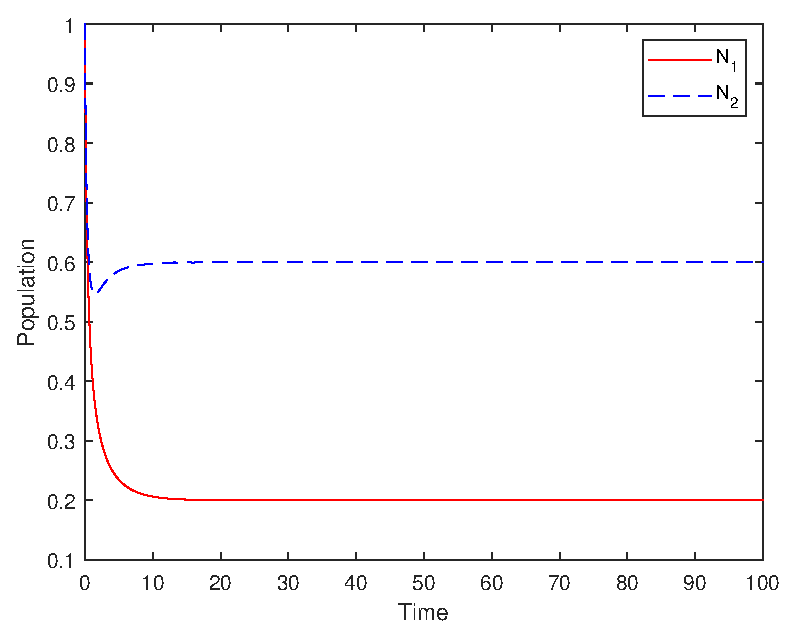
\includegraphics [width=4in]{ecologyComp_02.eps}\\
И тук двете популации запазват константен растеж във времето. \\
Тук стойността за $N_1$ е $0.2 = \frac{\Delta_1}{\Delta}$. \\
Аналогично за $N_2$ стойността е $0.6 = \frac{\Delta_2}{\Delta}$. \\
\newpage
\begin{figure}[htp!]
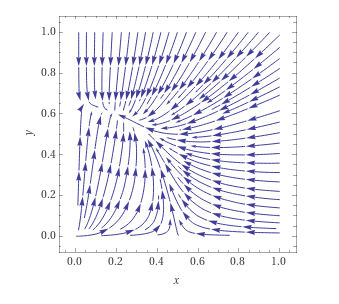
\includegraphics [width=6in]{fazof-portret-primer-2.png}
\caption{Фазов портет}
\end{figure}

















































\end{document}